\documentclass[aspectratio=169]{beamer}

% ──────────────────────────────────────────────
% PACKAGES
% ──────────────────────────────────────────────
\usepackage[utf8]{inputenc}
\usepackage[T1]{fontenc}
\usepackage{lmodern}
\usepackage{graphicx}
\usepackage{booktabs}
\usepackage{array}
\usepackage{xcolor}
\usepackage{tikz}
\usetikzlibrary{arrows.meta, positioning, shapes.geometric}
\usepackage{pgfplots}
\pgfplotsset{compat=1.18}
\usepackage{fontawesome5}
\usepackage{hyperref}
\usepackage{tcolorbox}
\tcbuselibrary{skins, breakable}
\usepackage{listings}
\usepackage{calc}

% ──────────────────────────────────────────────
% COLORS
% ──────────────────────────────────────────────
\definecolor{NavyBlue}{HTML}{1B2A4A}
\definecolor{TealPrimary}{HTML}{0D7377}
\definecolor{TealLight}{HTML}{14A085}
\definecolor{AccentCyan}{HTML}{32E0C4}
\definecolor{SlideGray}{HTML}{F4F6F9}
\definecolor{MutedGray}{HTML}{7A8FA6}
\definecolor{DarkText}{HTML}{1E293B}
\definecolor{LightCard}{HTML}{EEF2F7}
\definecolor{SuccessGreen}{HTML}{10B981}
\definecolor{WarnOrange}{HTML}{F59E0B}

% ──────────────────────────────────────────────
% BEAMER THEME SETUP
% ──────────────────────────────────────────────
\usetheme{default}
\usecolortheme{default}
\setbeamertemplate{navigation symbols}{}
\setbeamertemplate{itemize item}{\color{TealPrimary}\faAngleRight}
\setbeamertemplate{itemize subitem}{\color{AccentCyan}\small\faCircle}
\setbeamertemplate{enumerate item}{\color{NavyBlue}\textbf{\insertenumlabel.}}

% Fonts
\setbeamerfont{title}{size=\LARGE, series=\bfseries}
\setbeamerfont{subtitle}{size=\large, series=\mdseries}
\setbeamerfont{frametitle}{size=\large, series=\bfseries}
\setbeamerfont{framesubtitle}{size=\normalsize}
\setbeamerfont{footline}{size=\tiny}

% Colors
\setbeamercolor{title}{fg=white}
\setbeamercolor{subtitle}{fg=AccentCyan}
\setbeamercolor{background canvas}{bg=white}
\setbeamercolor{frametitle}{fg=white, bg=NavyBlue}
\setbeamercolor{item}{fg=TealPrimary}
\setbeamercolor{subitem}{fg=TealLight}
\setbeamercolor{block title}{fg=white, bg=TealPrimary}
\setbeamercolor{block body}{fg=DarkText, bg=LightCard}
\setbeamercolor{normal text}{fg=DarkText}

% Header bar
\setbeamertemplate{frametitle}{%
  \begin{beamercolorbox}[wd=\paperwidth, ht=0.65cm, dp=0.25cm, leftskip=0.4cm]{frametitle}
    \usebeamerfont{frametitle}\insertframetitle
    \ifx\insertframesubtitle\empty\else
      \hfill{\color{AccentCyan}\small\insertframesubtitle\hspace{0.4cm}}%
    \fi
  \end{beamercolorbox}
}

% Footer
\setbeamertemplate{footline}{%
  \begin{beamercolorbox}[wd=\paperwidth, ht=0.4cm, dp=0.15cm]{footline}
    \hspace{0.4cm}%
    {\color{MutedGray}\tiny HostelPulse --- Hostel Issue Management System%
    \hfill\color{TealPrimary}\tiny\insertframenumber/\inserttotalframenumber\hspace{0.3cm}}
  \end{beamercolorbox}
}

% Tcolorbox styles
\tcbset{
  infobox/.style={
    enhanced, colback=LightCard, colframe=TealPrimary,
    boxrule=0.5pt, arc=4pt, left=5pt, right=5pt, top=3pt, bottom=3pt,
    fontupper=\small\color{DarkText}
  },
  featurebox/.style={
    enhanced, colback=NavyBlue!8, colframe=NavyBlue,
    boxrule=0.5pt, arc=4pt, left=5pt, right=5pt, top=3pt, bottom=3pt,
    fontupper=\small\color{DarkText}
  },
  accentbox/.style={
    enhanced, colback=TealPrimary!10, colframe=AccentCyan,
    boxrule=0.8pt, arc=4pt, left=5pt, right=5pt, top=3pt, bottom=3pt,
    fontupper=\small\color{DarkText}
  }
}

% ──────────────────────────────────────────────
% TITLE SLIDE TEMPLATE (dark)
% ──────────────────────────────────────────────
\defbeamertemplate*{title page}{custom}{%
  \begin{tikzpicture}[remember picture, overlay]
    \fill[NavyBlue] (current page.south west) rectangle (current page.north east);
    \fill[TealPrimary] (current page.south west) rectangle ++(0.18\paperwidth, \paperheight);
    \fill[AccentCyan] (current page.south west) rectangle ++(0.04\paperwidth, \paperheight);
    \fill[TealLight, opacity=0.15] (current page.north east) ++(-1.2,-1.2) circle (2.4cm);
    \fill[AccentCyan, opacity=0.08] (current page.north east) ++(-1.8,-1.8) circle (1.5cm);
    \fill[TealPrimary, opacity=0.12] (current page.south east) ++(-0.8,1.2) circle (1.8cm);
  \end{tikzpicture}
  \vspace{0.5cm}
  \hspace{0.22\paperwidth}%
  \begin{minipage}{0.72\paperwidth}
    {\color{AccentCyan}\footnotesize\faBuilding\quad Mini Project Presentation}\\[0.25cm]
    {\color{white}\LARGE\bfseries HostelPulse}\\[0.1cm]
    {\color{AccentCyan!80!white}\large Hostel Issue Management System}\\[0.4cm]
    
\begin{tikzpicture}
      \draw[AccentCyan, line width=1pt] (0,0) -- (6cm,0);
    \end{tikzpicture}\\[0.35cm]
    {\color{white!80!NavyBlue}\footnotesize\bfseries GROUP MEMBERS}\\[0.15cm]
    {\color{white}\small
      Abhinav Singh \textcolor{MutedGray}{(2400520100004)}\\[0.04cm]
      Ansh Sharma \textcolor{MutedGray}{(2400520100016)}\\[0.04cm]
      Bhavya Nigam \textcolor{MutedGray}{(2400520100028)}\\[0.04cm]
      Devraj Gupta \textcolor{MutedGray}{(2400520100034)}\\[0.04cm]
      Himanshu \textcolor{MutedGray}{(2400520100040)}
    }\\[0.35cm]
    {\color{MutedGray}\footnotesize\faCalendar\quad 2025--2026
     \quad|\quad\faUniversity\quad IET Lucknow, CSE-R}
  \end{minipage}
}

% ──────────────────────────────────────────────
% DOCUMENT
% ──────────────────────────────────────────────
\begin{document}

% ── SLIDE 1: Title ─────────────────────────────
\begin{frame}[plain]
  \titlepage
\end{frame}

% ── SLIDE 2: Table of Contents ─────────────────
\begin{frame}{Outline}{}
  \begin{columns}[t]
    \column{0.5\textwidth}
    \begin{tcolorbox}[infobox, title={\color{white}\small\bfseries\faListAlt\quad Contents},
        colbacktitle=TealPrimary]
      \begin{enumerate}\setlength\itemsep{0.3em}
        \item Introduction
        \item Problem Statement \& Objectives
        \item System Flow \& Architecture
        \item Technology Stack
        \item Website Screenshots
        \item Database Design
        \item Conclusion
        \item References
      \end{enumerate}
    \end{tcolorbox}

    \column{0.45\textwidth}
    \vspace{0.2cm}
    \begin{tcolorbox}[accentbox]
      {\color{TealPrimary}\faInfoCircle}\quad
      {\small HostelPulse digitalizes hostel complaint management,
      replacing paper-based workflows with a transparent,
      role-based online system.}
    \end{tcolorbox}
    \vspace{0.25cm}
    \begin{tcolorbox}[featurebox]
      {\color{NavyBlue}\small\faUserGraduate}\quad{\small Students submit \& track issues}\\[4pt]
      {\color{NavyBlue}\small\faUserShield}\quad{\small Admin manages \& resolves them}\\[4pt]
      {\color{NavyBlue}\small\faCloud}\quad{\small Deployed on AWS}\\[4pt]
      {\color{NavyBlue}\small\faDatabase}\quad{\small MongoDB Atlas cloud database}
    \end{tcolorbox}
  \end{columns}
\end{frame}

% ── SLIDE 3: Introduction ───────────────────────
\begin{frame}{Introduction}{About the Project}
  \begin{columns}[t]
    \column{0.48\textwidth}
    \begin{tcolorbox}[infobox, title={\color{white}\small\bfseries What is HostelPulse?},
        colbacktitle=NavyBlue]
      {\small A \textbf{web-based platform} built to streamline
      reporting and resolution of hostel-related issues for
      students and administrators.\\[5pt]
      Students raise complaints online and track their status
      in real time, while wardens manage and resolve them
      through a centralized dashboard.}
    \end{tcolorbox}
    \vspace{0.25cm}
    \begin{tcolorbox}[accentbox]
      {\small\textbf{Target Users:}\quad
      {\color{TealPrimary}\faUserGraduate}\ Students \quad
      {\color{NavyBlue}\faUserShield}\ Admin/Warden}
    \end{tcolorbox}

    \column{0.48\textwidth}
    \begin{tcolorbox}[featurebox, title={\color{white}\small\bfseries Key Highlights},
        colbacktitle=TealPrimary]
      \begin{itemize}\setlength\itemsep{0.25em}
        \item[\color{AccentCyan}\faCheckCircle] Online complaint submission portal
        \item[\color{AccentCyan}\faCheckCircle] Role-based access (Student / Admin)
        \item[\color{AccentCyan}\faCheckCircle] Real-time issue status tracking
        \item[\color{AccentCyan}\faCheckCircle] Admin dashboard for management
        \item[\color{AccentCyan}\faCheckCircle] JWT-secured authentication
        \item[\color{AccentCyan}\faCheckCircle] MongoDB cloud database
        \item[\color{AccentCyan}\faCheckCircle] Deployed fully on AWS
      \end{itemize}
    \end{tcolorbox}
  \end{columns}
\end{frame}

% ── SLIDE 4: Problem Statement ─────────────────
\begin{frame}{Problem Statement \& Objectives}{}
  \begin{columns}[t]
    \column{0.48\textwidth}
    \begin{tcolorbox}[enhanced, colback=red!5, colframe=red!50!NavyBlue,
        boxrule=0.5pt, arc=4pt, left=5pt, right=5pt, top=3pt, bottom=3pt,
        title={\color{white}\small\bfseries\faExclamationTriangle\quad Problems},
        colbacktitle=red!60!NavyBlue,
        fontupper=\small\color{DarkText}]
      \begin{itemize}\setlength\itemsep{0.22em}
        \item Complaints reported manually on paper
        \item No centralized tracking system
        \item No accountability for resolution
        \item Students unaware of complaint status
        \item Difficult to identify recurring issues
        \item Warden overload from verbal complaints
      \end{itemize}
    \end{tcolorbox}

    \column{0.48\textwidth}
    \begin{tcolorbox}[enhanced, colback=SuccessGreen!6, colframe=SuccessGreen!70,
        boxrule=0.5pt, arc=4pt, left=5pt, right=5pt, top=3pt, bottom=3pt,
        title={\color{white}\small\bfseries\faBullseye\quad Objectives},
        colbacktitle=TealPrimary,
        fontupper=\small\color{DarkText}]
      \begin{itemize}\setlength\itemsep{0.22em}
        \item Build a digital complaint submission portal
        \item Provide real-time status updates to students
        \item Enable admin to manage issues centrally
        \item Implement role-based secure authentication
       
        \item Reduce manual workload through automation
      \end{itemize}
    \end{tcolorbox}
  \end{columns}
\end{frame}

% ── SLIDE 5: System Flow ────────────────────────
\begin{frame}{System Flow \& Architecture}{}
  \begin{columns}[T]
    \column{0.50\textwidth}
    \vspace{0.15cm}
    \begin{center}
    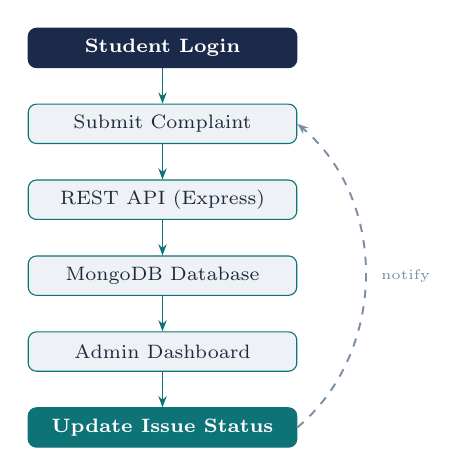
\begin{tikzpicture}[
        node distance=0.45cm,
        box/.style={
          rectangle, rounded corners=3pt,
          draw=TealPrimary, fill=LightCard,
          text width=3.2cm, align=center,
          font=\scriptsize\color{DarkText},
          minimum height=0.5cm, inner sep=3pt
        },
        darkbox/.style={
          rectangle, rounded corners=3pt,
          draw=NavyBlue, fill=NavyBlue,
          text width=3.2cm, align=center,
          font=\scriptsize\bfseries\color{white},
          minimum height=0.5cm, inner sep=3pt
        },
        tealbox/.style={
          rectangle, rounded corners=3pt,
          draw=TealPrimary, fill=TealPrimary,
          text width=3.2cm, align=center,
          font=\scriptsize\bfseries\color{white},
          minimum height=0.5cm, inner sep=3pt
        },
        arr/.style={-{Stealth[length=4pt]}, TealPrimary, line width=0.7pt}
      ]
      \node[darkbox]               (login)   {Student Login};
      \node[box, below=of login]   (submit)  {Submit Complaint};
      \node[box, below=of submit]  (api)     {REST API (Express)};
      \node[box, below=of api]     (db)      {MongoDB Database};
      \node[box, below=of db]      (admin)   {Admin Dashboard};
      \node[tealbox, below=of admin] (resolve) {Update Issue Status};

      \draw[arr] (login)   -- (submit);
      \draw[arr] (submit)  -- (api);
      \draw[arr] (api)     -- (db);
      \draw[arr] (db)      -- (admin);
      \draw[arr] (admin)   -- (resolve);
      \draw[-{Stealth[length=4pt]}, MutedGray, dashed, line width=0.7pt,
            bend right=50]
            (resolve.east) to
            node[right, font=\tiny\color{MutedGray}, xshift=2pt]
            {notify} (submit.east);
    \end{tikzpicture}
    \end{center}

    \column{0.46\textwidth}
    \vspace{0.2cm}
    \begin{tcolorbox}[infobox,
        title={\color{white}\small\bfseries\faUserGraduate\ Student Actions},
        colbacktitle=TealLight]
      \begin{itemize}\setlength\itemsep{0.18em}
        \item Register and login securely
        \item Submit hostel complaints
        \item Track complaint status
        \item Edit or delete own issues
      \end{itemize}
    \end{tcolorbox}
    \vspace{0.2cm}
    \begin{tcolorbox}[infobox,
        title={\color{white}\small\bfseries\faUserShield\ Admin / Warden Actions},
        colbacktitle=NavyBlue]
      \begin{itemize}\setlength\itemsep{0.18em}
        \item View all complaints
        \item Update issue status
       
      \end{itemize}
    \end{tcolorbox}
  \end{columns}
\end{frame}

% ── SLIDE 6: Technology Stack ───────────────────
\begin{frame}{Technology Stack}{}
  \begin{columns}[t]
    \column{0.24\textwidth}
    \begin{tcolorbox}[infobox, title={\color{white}\small\bfseries\faCode\ Frontend},
        colbacktitle=TealPrimary, height=4.2cm]
      \textbf{React.js}\\
      {\tiny Component-based UI}\\[5pt]
      \textbf{Tailwind CSS}\\
      {\tiny Utility-first styling}\\[5pt]
      \textbf{Axios}\\
      {\tiny HTTP client}
    \end{tcolorbox}

    \column{0.24\textwidth}
    \begin{tcolorbox}[infobox, title={\color{white}\small\bfseries\faServer\ Backend},
        colbacktitle=TealPrimary, height=4.2cm]
      \textbf{Node.js}\\
      {\tiny JS runtime}\\[5pt]
      \textbf{Express.js}\\
      {\tiny REST API framework}\\[5pt]
      \textbf{JWT + bcrypt}\\
      {\tiny Auth \& hashing}
    \end{tcolorbox}

    \column{0.24\textwidth}
    \begin{tcolorbox}[infobox, title={\color{white}\small\bfseries\faDatabase\ Database},
        colbacktitle=TealPrimary, height=4.2cm]
      \textbf{MongoDB Atlas}\\
      {\tiny Cloud NoSQL DB}\\[5pt]
      \textbf{Mongoose}\\
      {\tiny ODM for Node}\\[5pt]
      \textbf{Schema Validation}\\
      {\tiny Strict type checks}
    \end{tcolorbox}

    \column{0.24\textwidth}
    \begin{tcolorbox}[infobox, title={\color{white}\small\bfseries\faCloud\ Deployment},
        colbacktitle=NavyBlue, height=4.2cm]
      \textbf{AWS}\\
      {\tiny Frontend \& Backend}\\[5pt]
      \textbf{Git / GitHub}\\
      {\tiny Source control}\\[5pt]
      \textbf{MongoDB Atlas}\\
      {\tiny Cloud database}
    \end{tcolorbox}
  \end{columns}
  \vspace{0.15cm}
  \begin{tcolorbox}[accentbox, left=8pt, right=8pt]
    {\color{NavyBlue}\faGithub}\quad
    {\small\textbf{Repo:}\ \texttt{https://github.com/ietlucknowofficial/HostelPulse}}
    \hfill
    {\color{TealPrimary}\faCloud}\quad
    {\small\textbf{Hosted on AWS}}
  \end{tcolorbox}
\end{frame}

% ── SLIDE 7: Screenshots --- Home & Student ────
\begin{frame}{Website Screenshots}{Home \& Student View}
  \begin{columns}[t]
    \column{0.48\textwidth}
    \begin{tcolorbox}[infobox, title={\color{white}\small\bfseries Home Page},
        colbacktitle=NavyBlue]
      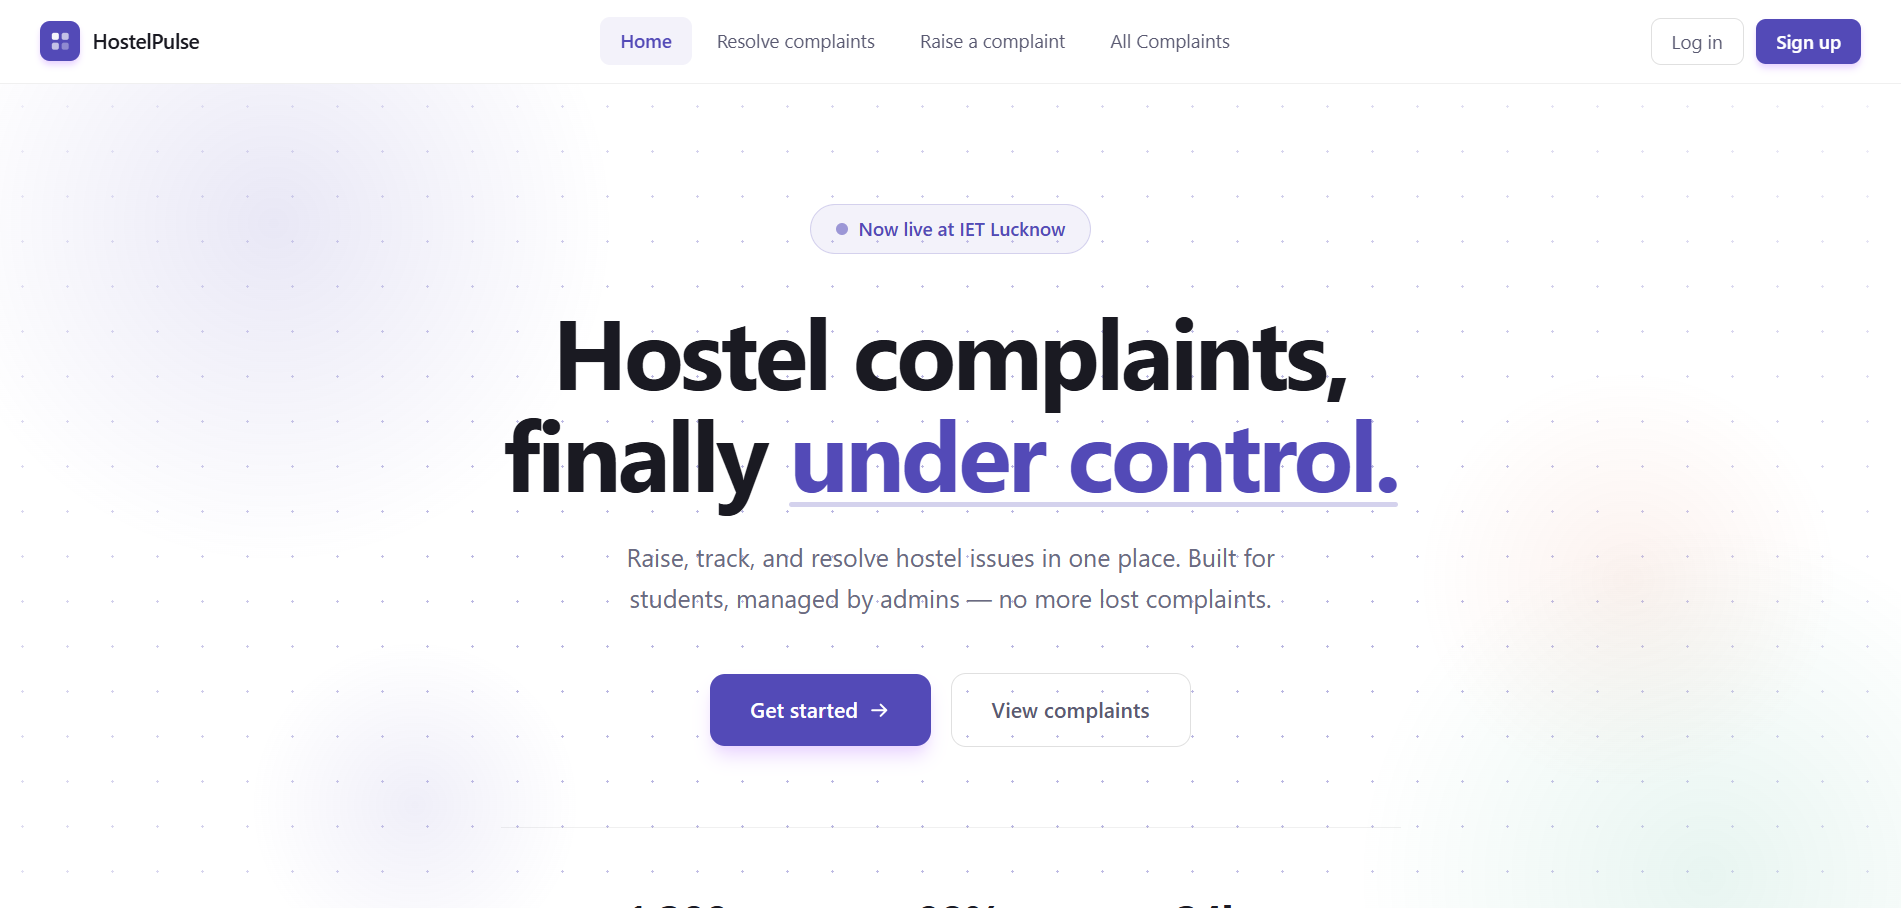
\includegraphics[width=\linewidth]{Home.png}\\[-2pt]
      {\tiny Landing page with login \& registration}
    \end{tcolorbox}

    \column{0.48\textwidth}
    \begin{tcolorbox}[infobox, title={\color{white}\small\bfseries Student Dashboard},
        colbacktitle=NavyBlue]
      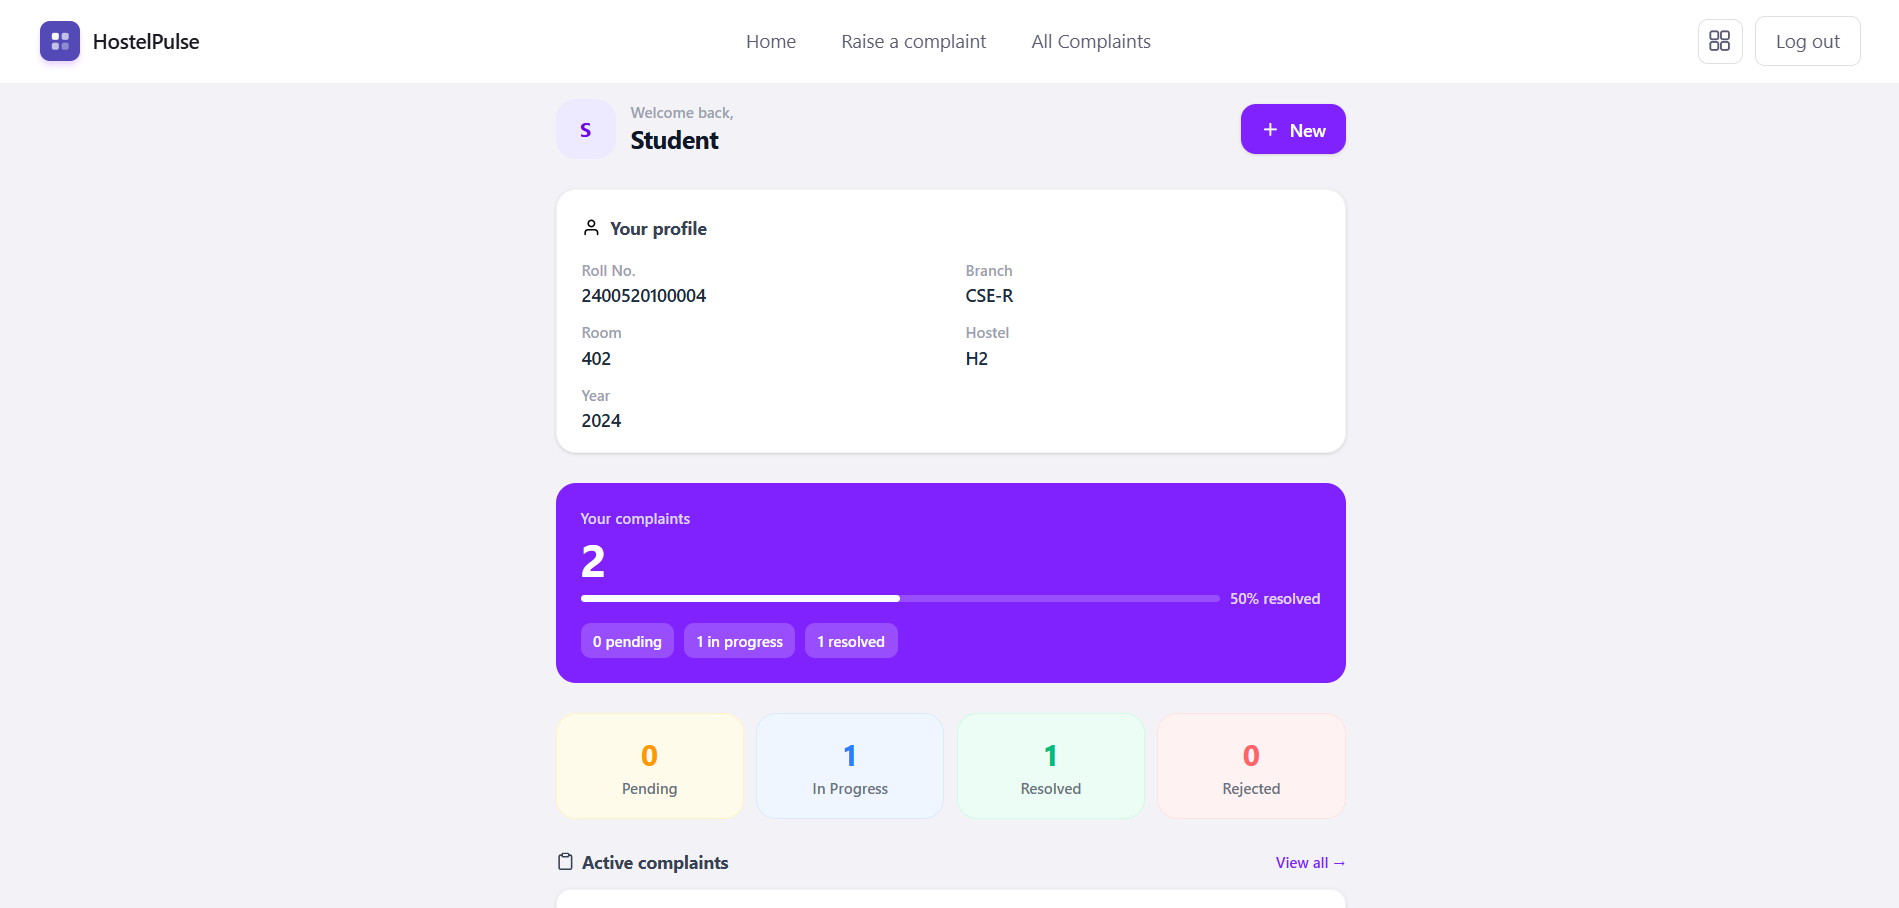
\includegraphics[width=\linewidth]{StudentDashboard.png}\\[-2pt]
      {\tiny Student complaint tracking dashboard}
    \end{tcolorbox}
  \end{columns}
\end{frame}

% ── SLIDE 8: Screenshots --- Admin & Form ──────
\begin{frame}{Website Screenshots}{Admin Panel \& Complaint Form}
  \begin{columns}[t]
    \column{0.48\textwidth}
    \begin{tcolorbox}[infobox, title={\color{white}\small\bfseries Admin Dashboard},
        colbacktitle=NavyBlue]
      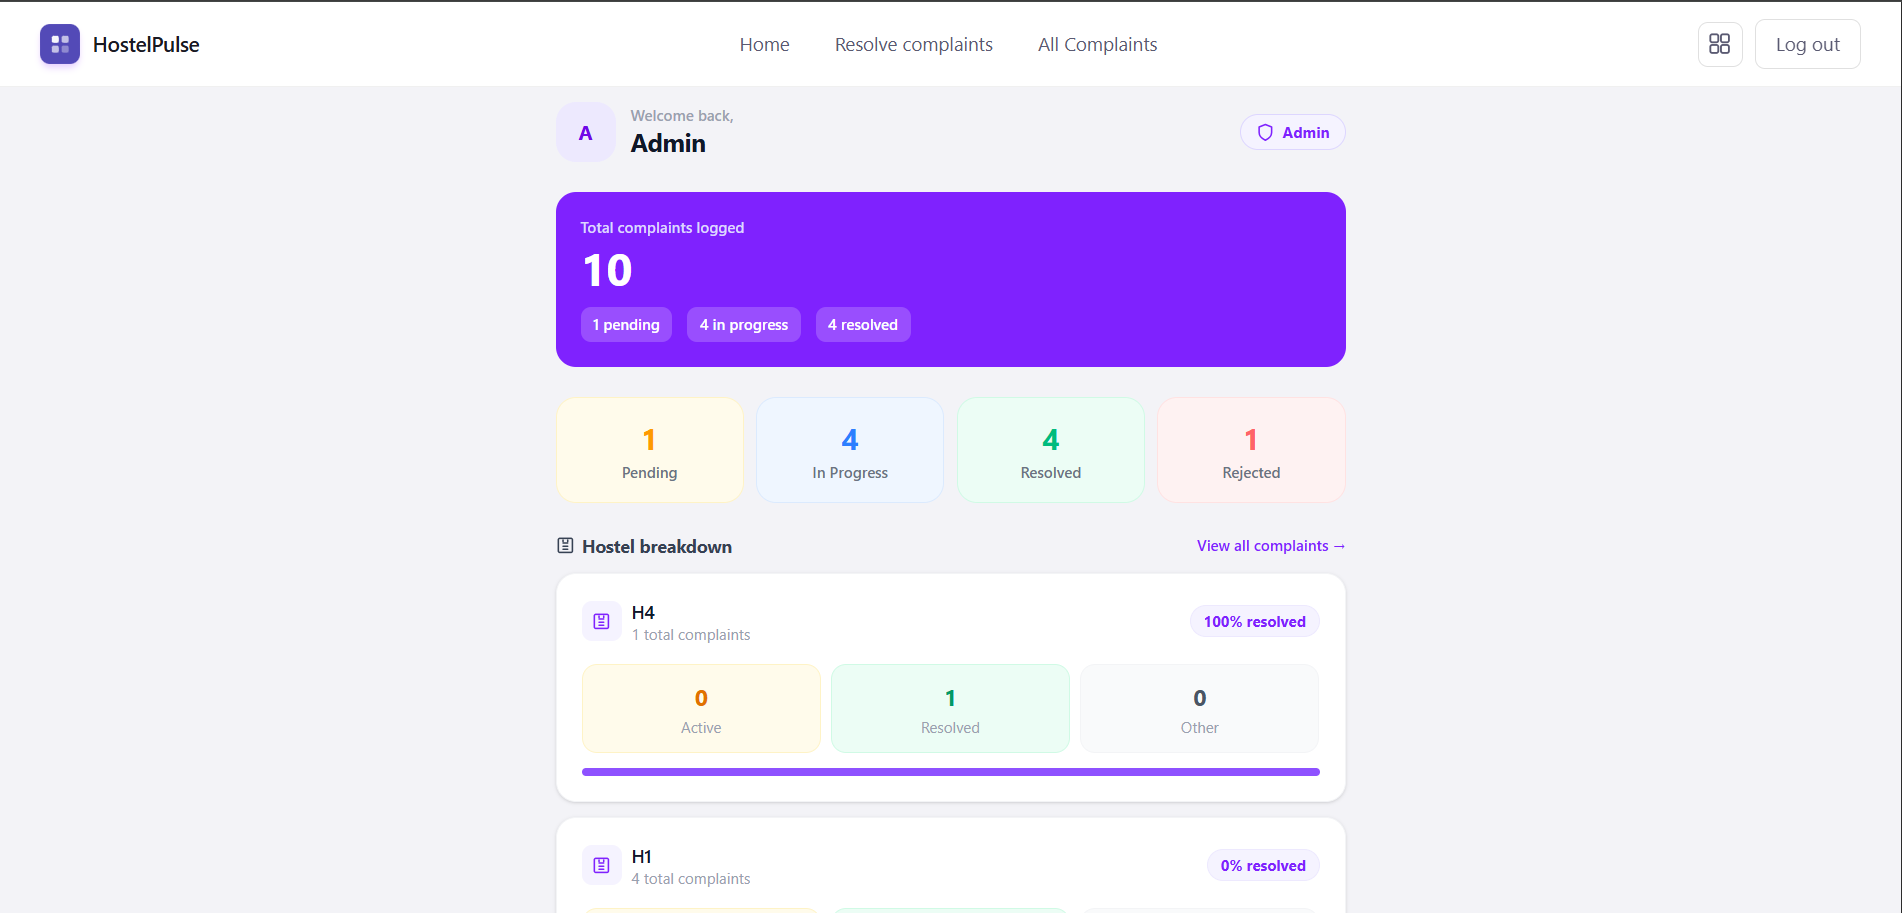
\includegraphics[width=\linewidth]{AdminDashboard.png}\\[-2pt]
      {\tiny Centralized admin panel with statistics}
    \end{tcolorbox}

    \column{0.48\textwidth}
    \begin{tcolorbox}[infobox, title={\color{white}\small\bfseries Submit Complaint Form},
        colbacktitle=NavyBlue]
      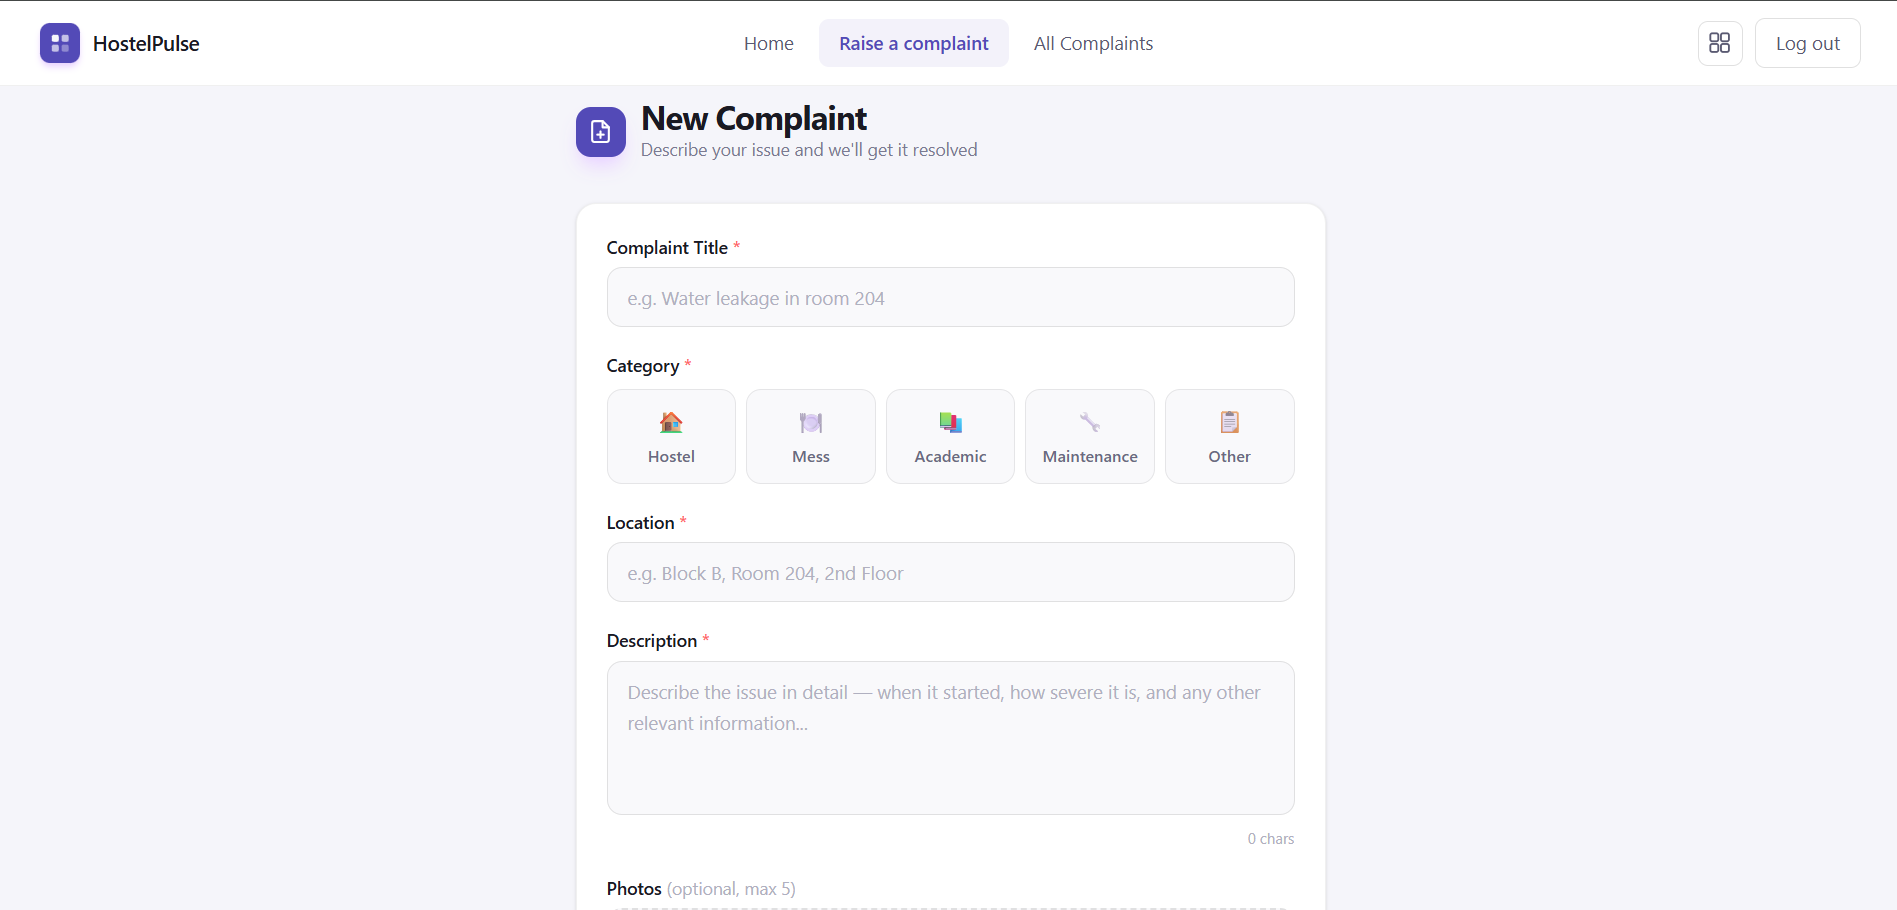
\includegraphics[width=\linewidth]{ComplaintForm.png}\\[-2pt]
      {\tiny Structured form with category \& room details}
    \end{tcolorbox}
  \end{columns}
\end{frame}

% ── SLIDE 9: Screenshots --- Complaints Lists ──
\begin{frame}{Website Screenshots}{Complaints Management}
  \begin{columns}[t]
    \column{0.48\textwidth}
    \begin{tcolorbox}[infobox, title={\color{white}\small\bfseries Complaints List (Admin)},
        colbacktitle=NavyBlue]
      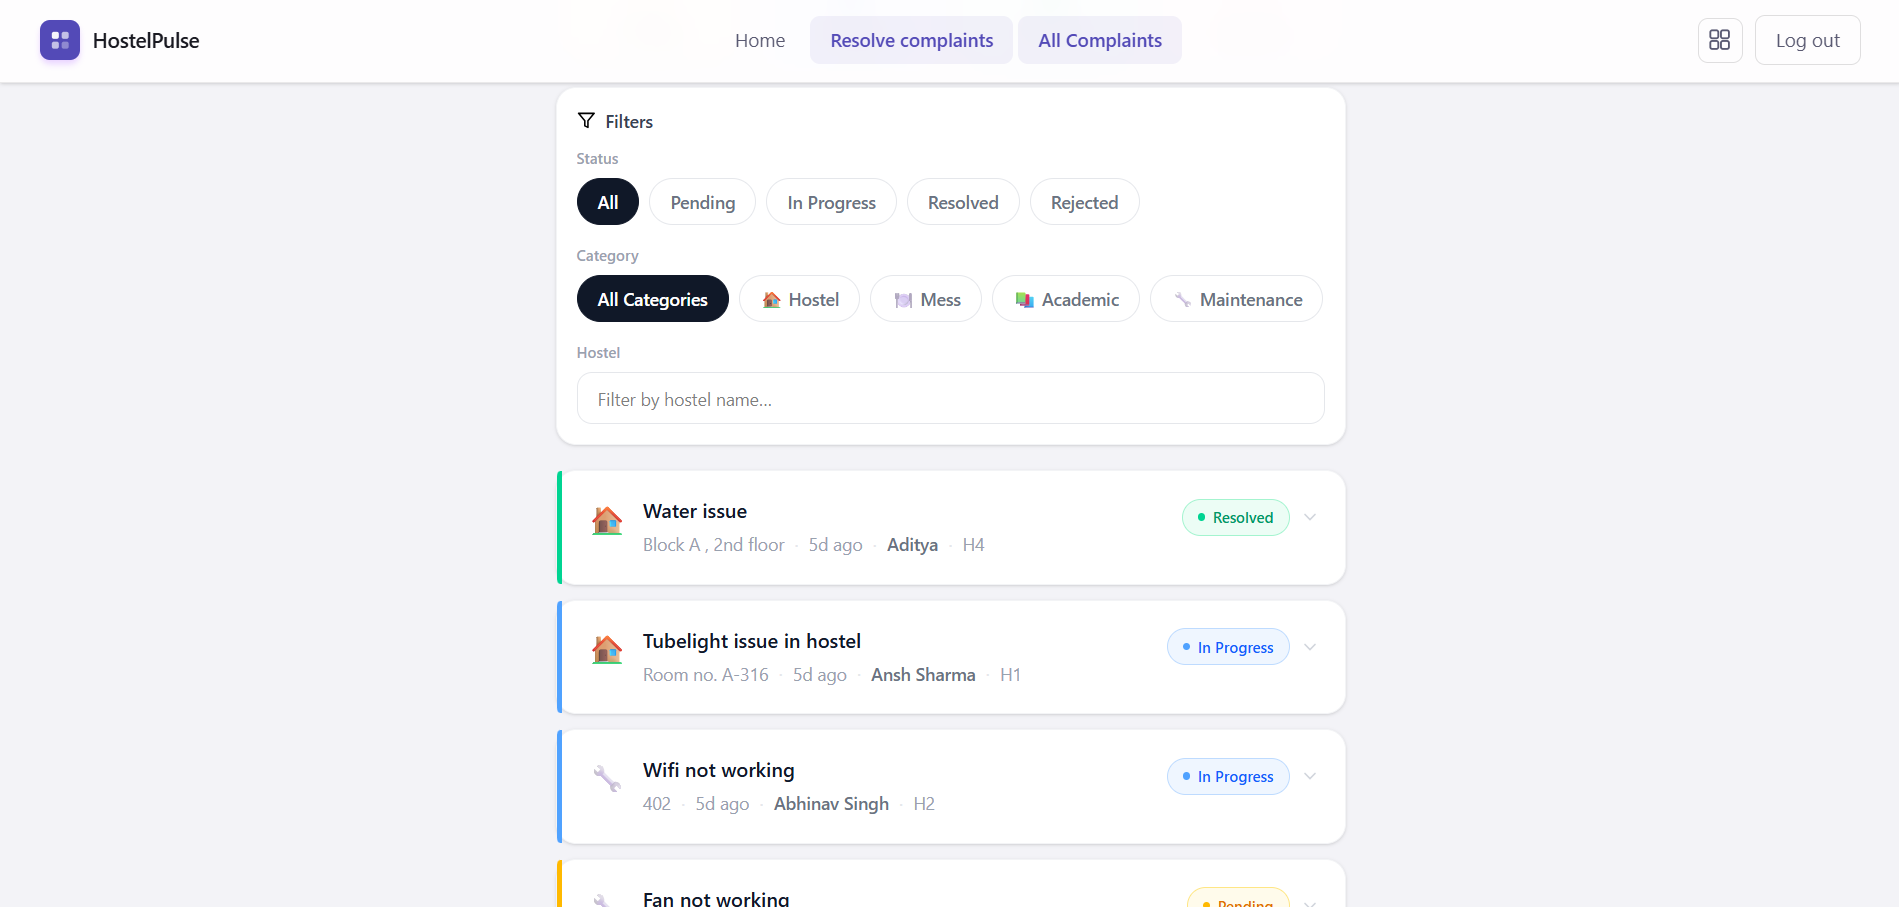
\includegraphics[width=\linewidth]{ComplaintsListAdmin.png}\\[-2pt]
      {\tiny Admin view: manage all student issues}
    \end{tcolorbox}

    \column{0.48\textwidth}
    \begin{tcolorbox}[infobox, title={\color{white}\small\bfseries Complaints List (Student)},
        colbacktitle=NavyBlue]
      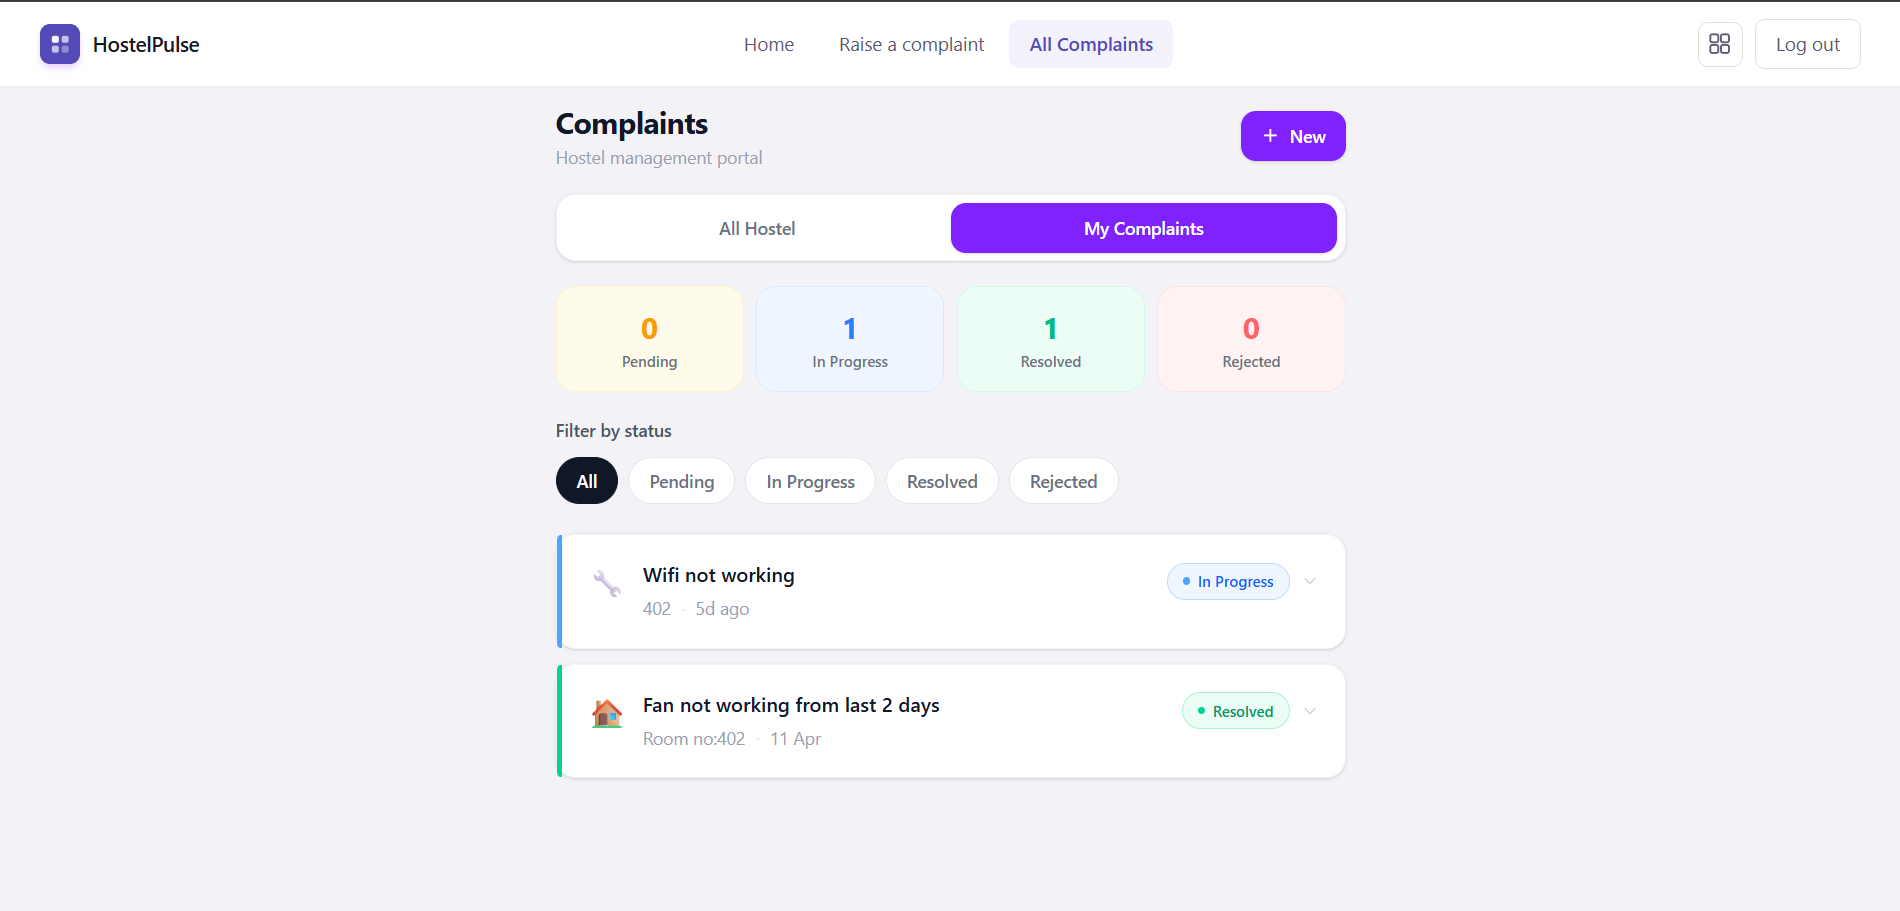
\includegraphics[width=\linewidth]{ComplaintsList.png}\\[-2pt]
      {\tiny All complaints submitted by a student}
    \end{tcolorbox}
  \end{columns}
\end{frame}

% ── SLIDE 10: Database Screenshots ─────────────
\begin{frame}{Website Screenshots}{Complaint Database \& User Collection}
  \begin{columns}[t]
    \column{0.48\textwidth}
    \begin{tcolorbox}[infobox, title={\color{white}\small\bfseries Complaint Database},
        colbacktitle=NavyBlue]
      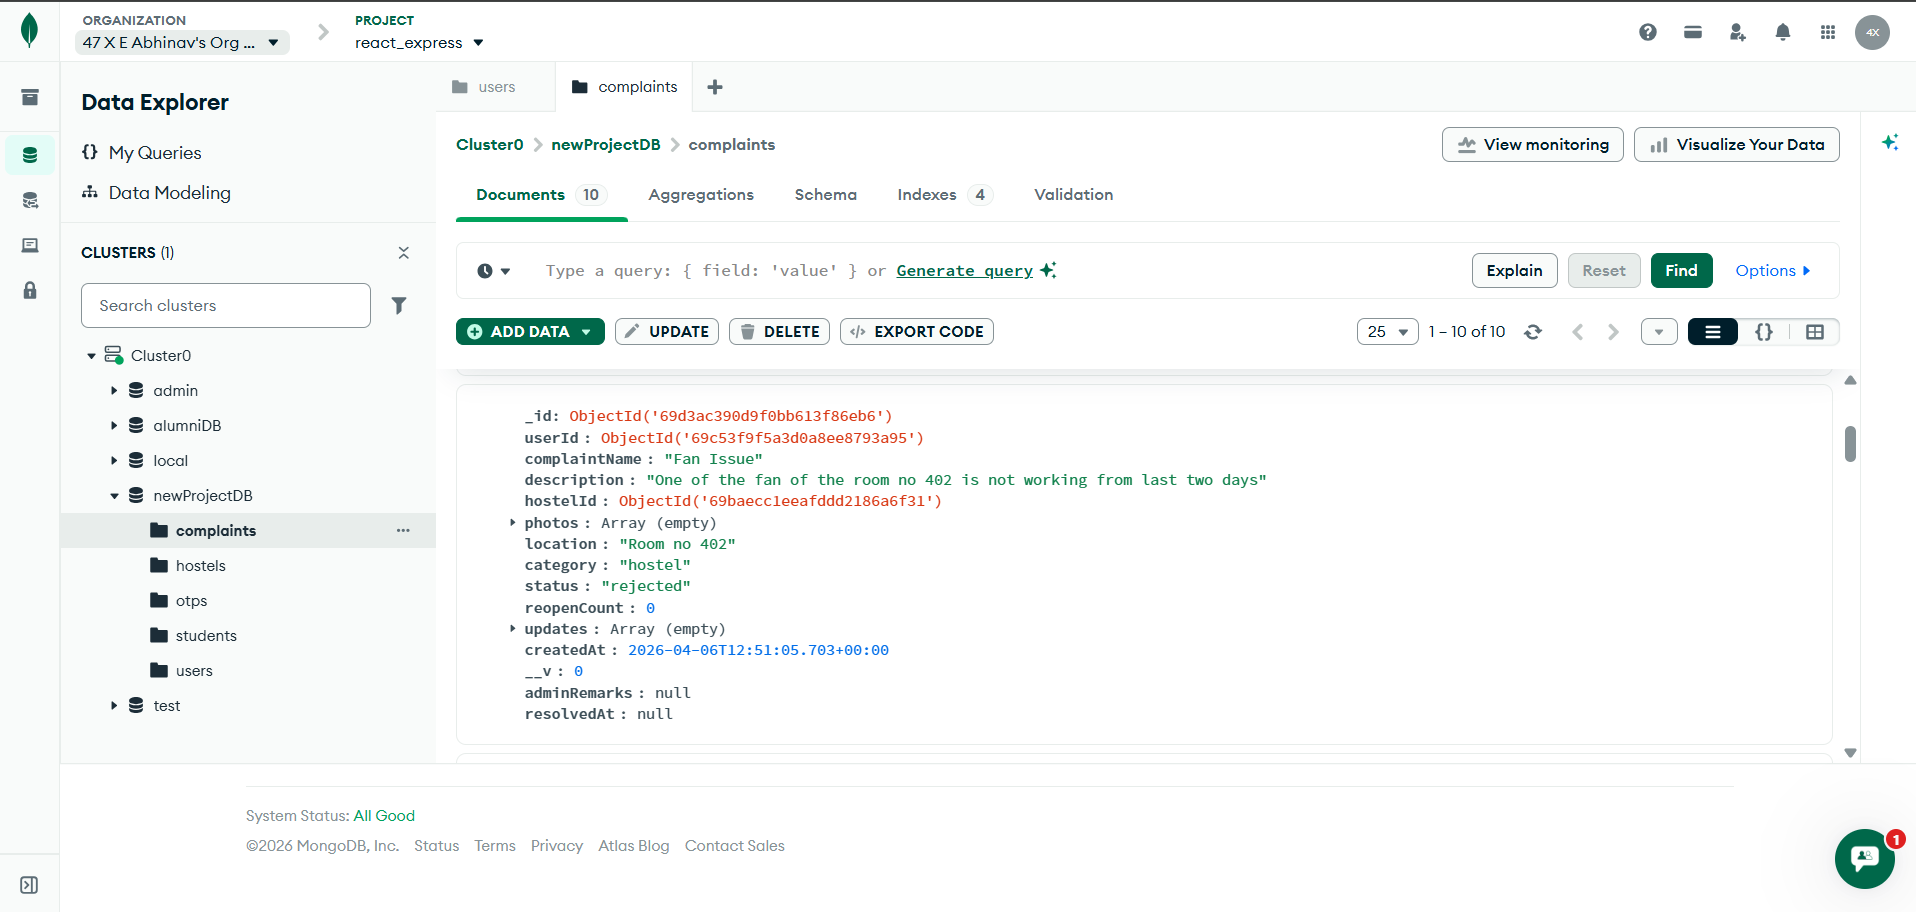
\includegraphics[width=\linewidth]{Complaints.png}\\[-2pt]
      {\tiny Complaints collection in MongoDB Atlas}
    \end{tcolorbox}

    \column{0.48\textwidth}
    \begin{tcolorbox}[infobox, title={\color{white}\small\bfseries User Collection},
        colbacktitle=NavyBlue]
      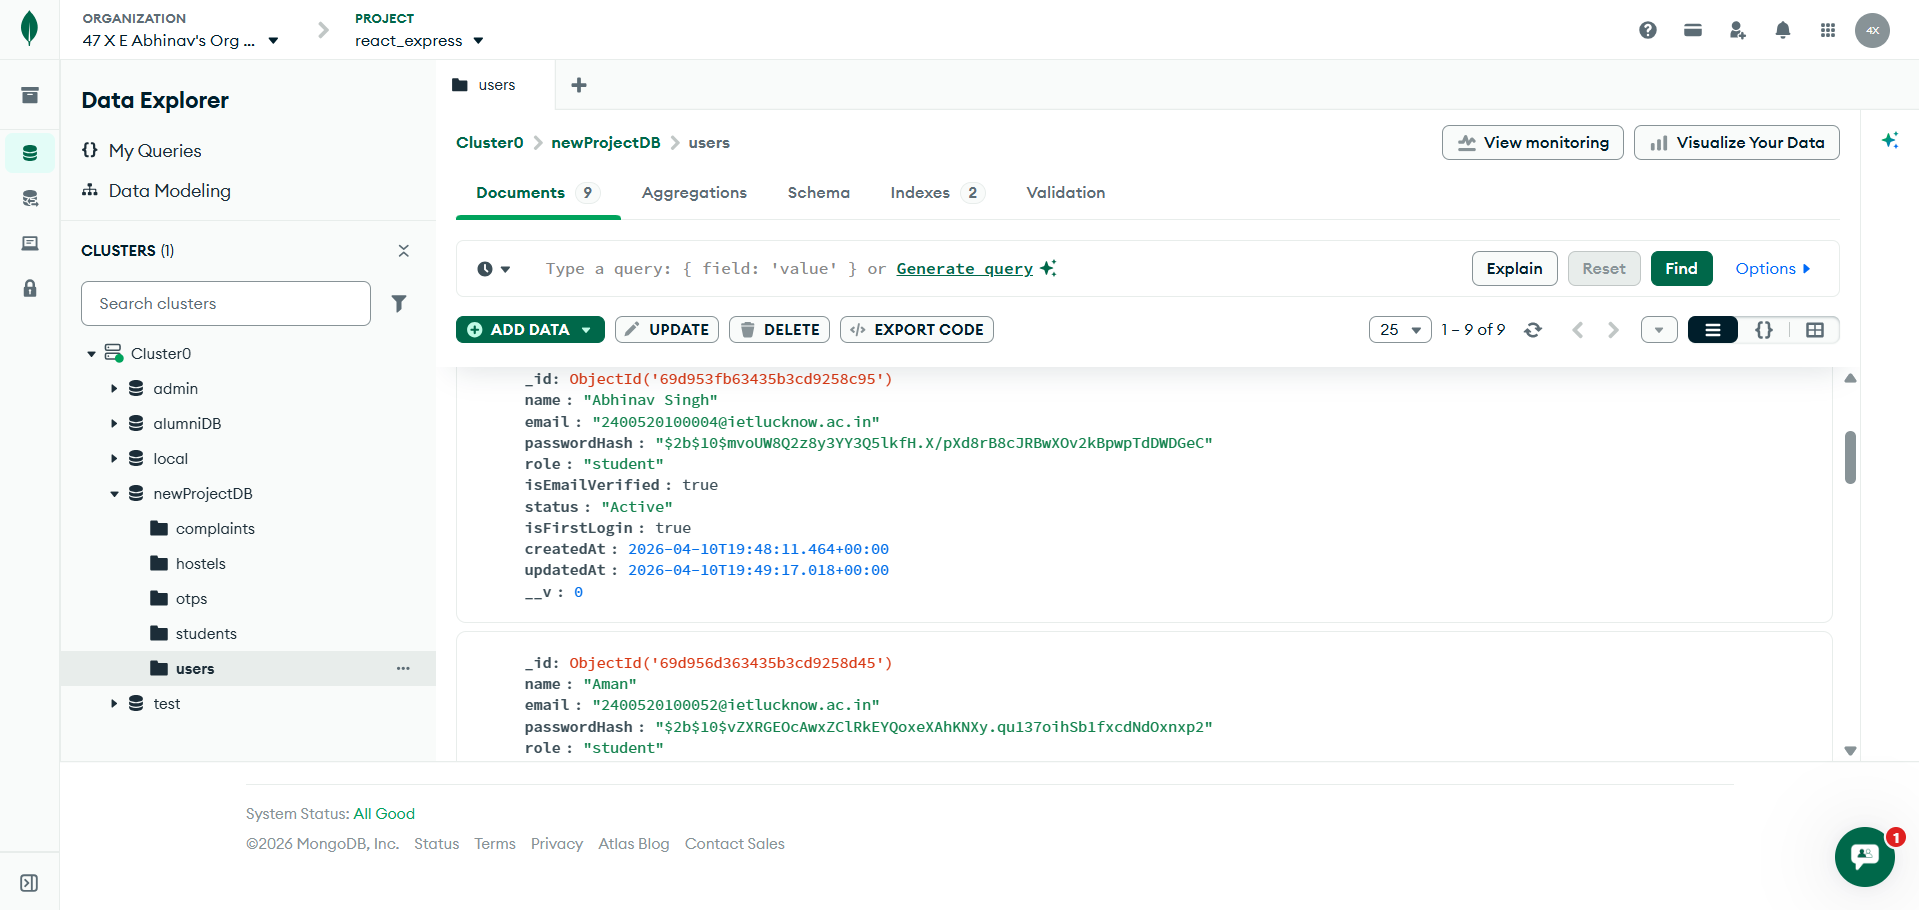
\includegraphics[width=\linewidth]{Users.png}\\[-2pt]
      {\tiny Users collection in MongoDB Atlas}
    \end{tcolorbox}
  \end{columns}
\end{frame}

% ── SLIDE 11: Database Design ───────────────────
\begin{frame}{Database Design}{MongoDB Collections}
  \begin{columns}[t]
    \column{0.48\textwidth}
    \begin{tcolorbox}[infobox,
        title={\color{white}\small\bfseries\faDatabase\ Students Collection},
        colbacktitle=NavyBlue]
      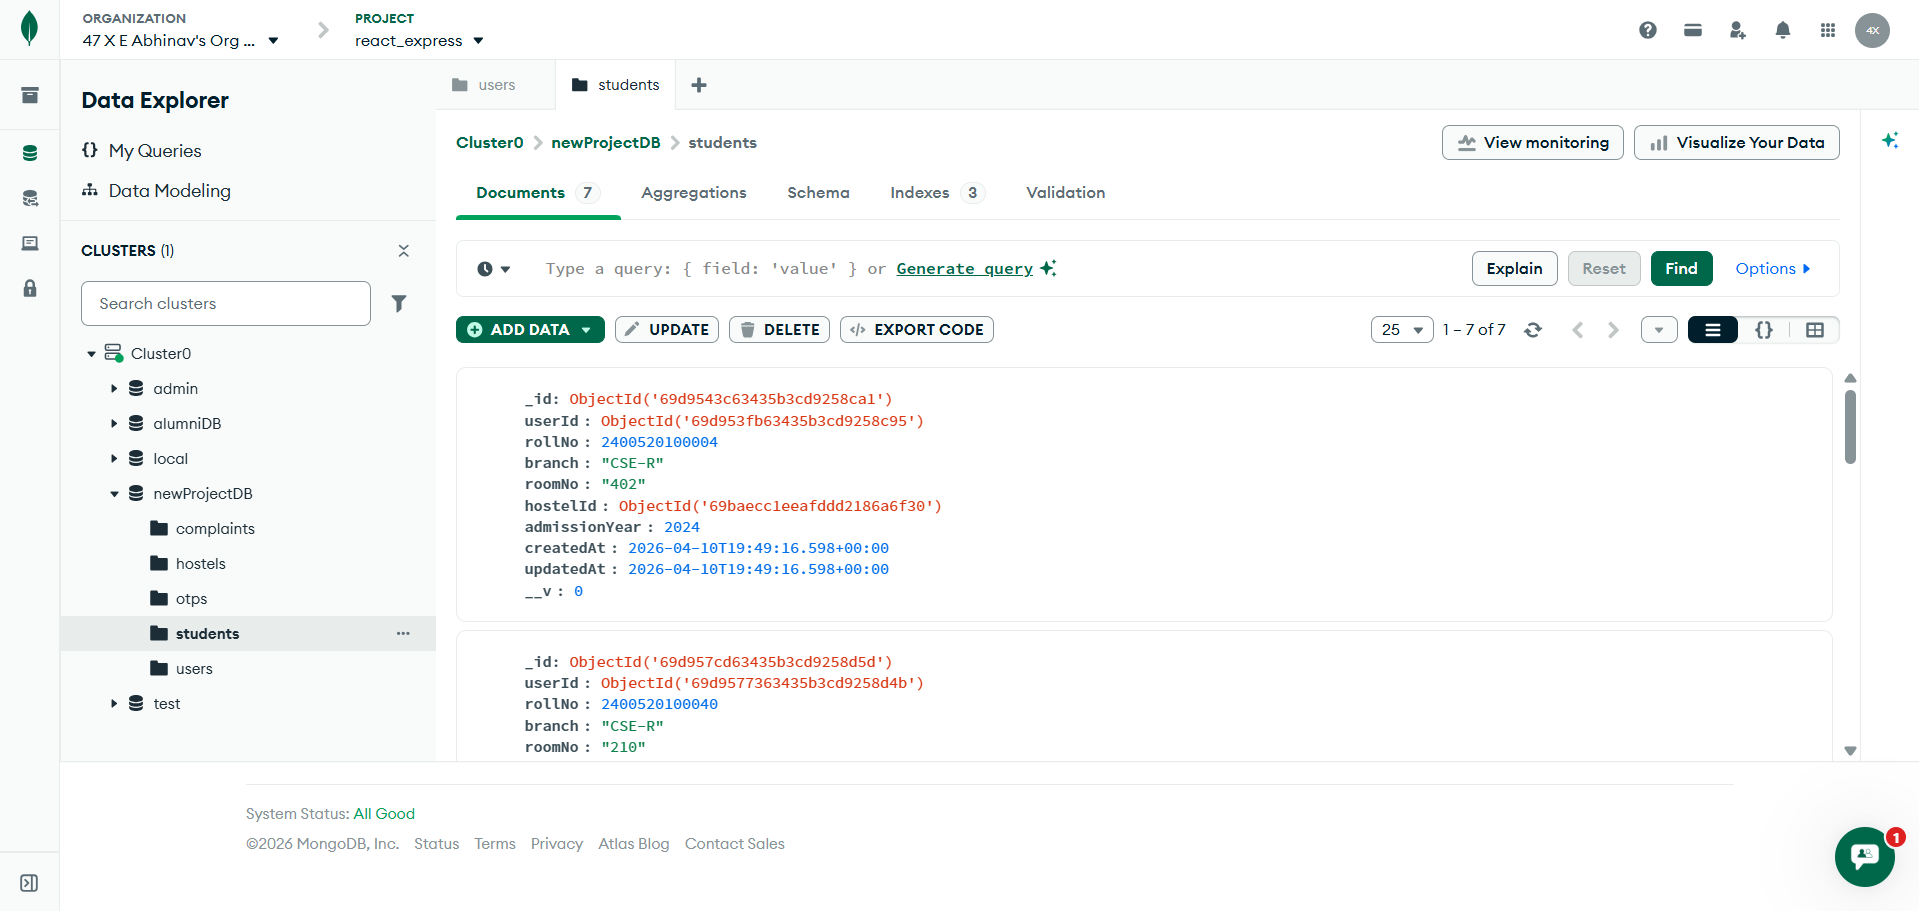
\includegraphics[width=\linewidth]{Students.png}\\[-2pt]
      {\tiny Students collection stored in MongoDB Atlas}
    \end{tcolorbox}

    \column{0.48\textwidth}
    \begin{tcolorbox}[infobox,
        title={\color{white}\small\bfseries\faDatabase\ Collection Fields},
        colbacktitle=TealPrimary]
      {\small\textbf{users} collection:}
      \begin{itemize}\setlength\itemsep{0.12em}
        {\scriptsize
        \item \texttt{\_id,\ name,\ email}
        \item \texttt{password} (bcrypt hashed)
        \item \texttt{role}: student $|$ admin
        \item \texttt{rollNo,\ roomNo,\ isVerified}
        }
      \end{itemize}
      \vspace{4pt}
      {\small\textbf{complaints} collection:}
      \begin{itemize}\setlength\itemsep{0.12em}
        {\scriptsize
        \item \texttt{\_id,\ userId} (ref to user)
        \item \texttt{title,\ description,\ category}
        \item \texttt{roomNo}
        \item \texttt{status}: pending $|$ resolved
        \item \texttt{createdAt,\ updatedAt}
        }
      \end{itemize}
    \end{tcolorbox}
  \end{columns}
\end{frame}

% ── SLIDE 12: Comparison Table ─────────────────

% ── SLIDE 13: Conclusion ────────────────────────
\begin{frame}{Conclusion}{}
  \begin{columns}[t]
    \column{0.48\textwidth}
    \begin{tcolorbox}[infobox, title={\color{white}\small\bfseries\faFlag\ Summary},
        colbacktitle=TealPrimary]
      {\small HostelPulse successfully digitalizes the hostel
      complaint process with a secure, scalable MERN
      application. It provides:}
      \begin{itemize}\setlength\itemsep{0.2em}
        \item Faster complaint resolution
        \item Transparent communication
        \item Reduced manual workload
        \item Centralized hostel management
        \item Better monitoring of recurring issues
      \end{itemize}
    \end{tcolorbox}

    \column{0.48\textwidth}
    \begin{tcolorbox}[featurebox,
        title={\color{white}\small\bfseries\faRocket\ Future Enhancements},
        colbacktitle=NavyBlue]
      \begin{itemize}\setlength\itemsep{0.25em}
        \item Push notifications (email / SMS)
        \item Analytics dashboard with charts
        \item Mobile app (React Native)
        \item Multi-hostel / multi-campus support
        \item Complaint priority levels
        \item Scheduled maintenance alerts
      \end{itemize}
    \end{tcolorbox}
    \vspace{0.2cm}
    \begin{tcolorbox}[accentbox]
      {\color{TealPrimary}\small\faGithub}\
      {\small\texttt{https://github.com/ietlucknowofficial/HostelPulse}}\\[3pt]
      {\color{TealPrimary}\small\faCloud}\
      {\small\texttt{https://d1fwtw1io6mluw.cloudfront.net/}}
    \end{tcolorbox}
  \end{columns}
\end{frame}

% ── SLIDE 14: References ────────────────────────
\begin{frame}{References}{}
  \begin{columns}[t]
    \column{0.55\textwidth}
    \begin{tcolorbox}[infobox,
        title={\color{white}\small\bfseries\faBook\ Documentation \& Resources},
        colbacktitle=NavyBlue]
      \begin{enumerate}\setlength\itemsep{0.28em}
        {\small
        \item React.js Official Docs --- \texttt{react.dev}
        \item Node.js Documentation --- \texttt{nodejs.org/docs}
        \item Express.js Guide --- \texttt{expressjs.com}
        \item MongoDB Atlas Docs --- \texttt{mongodb.com/docs}
        \item JWT Standard (RFC~7519) --- \texttt{jwt.io}
        \item AWS Documentation --- \texttt{docs.aws.amazon.com}
        \item Tailwind CSS Docs --- \texttt{tailwindcss.com}
        }
      \end{enumerate}
    \end{tcolorbox}

    \column{0.41\textwidth}
    \begin{tcolorbox}[accentbox,
        title={\color{white}\small\bfseries\faLink\ Project Links},
        colbacktitle=TealPrimary]
      {\small
      \textbf{GitHub Repository:}\\[2pt]
      {\footnotesize\texttt{https://github.com/ietlucknowofficial/HostelPulse}}\\[8pt]
      \textbf{Hosted on AWS:}\\[2pt]
      {\footnotesize\texttt{https://d1fwtw1io6mluw.cloudfront.net/}}
      }
    \end{tcolorbox}
    \vspace{0.2cm}
    \begin{tcolorbox}[featurebox]
      {\small\color{MutedGray}
       \faCode\quad Built with the MERN Stack\\[3pt]
       \faUniversity\quad IET Lucknow, CSE-R\\[3pt]
       \faCalendar\quad Academic Year 2025--26}
    \end{tcolorbox}
  \end{columns}
\end{frame}

% ── SLIDE 15: Thank You ─────────────────────────
\begin{frame}[plain]
  \begin{tikzpicture}[remember picture, overlay]
    \fill[NavyBlue] (current page.south west) rectangle (current page.north east);
    \fill[TealPrimary] (current page.south west) rectangle ++(0.18\paperwidth, \paperheight);
    \fill[AccentCyan] (current page.south west) rectangle ++(0.04\paperwidth, \paperheight);
    \fill[TealLight, opacity=0.1] (current page.north east) ++(-1.5,-1.5) circle (3cm);
    \fill[AccentCyan, opacity=0.07] (current page.south east) ++(-1,1.5) circle (2cm);
  \end{tikzpicture}

  \vspace{1.3cm}
  \hspace{0.22\paperwidth}%
  \begin{minipage}{0.7\paperwidth}
    {\color{AccentCyan}\Large\bfseries Thank You!}\\[0.35cm]
    
\begin{tikzpicture}
      \draw[AccentCyan, line width=1pt] (0,0) -- (5cm,0);
    \end{tikzpicture}\\[0.35cm]
    {\color{white}\large\bfseries Questions \& Discussion}\\[0.5cm]
    {\color{white!70!NavyBlue}\small
      Abhinav Singh\ \textbullet\ Ansh Sharma\ \textbullet\ Bhavya Nigam\\[2pt]
      Devraj Gupta\ \textbullet\ Himanshu\\[0.4cm]
    }
    {\color{AccentCyan}\small\faGithub}\
    {\color{white}\small\texttt{https://github.com/ietlucknowofficial/HostelPulse}}\\[0.2cm]
    {\color{AccentCyan}\small\faCloud}\
    {\color{white}\small\texttt{https://d1fwtw1io6mluw.cloudfront.net/}}\\[0.2cm]
    {\color{AccentCyan}\small\faUniversity}\
    {\color{white}\small IET Lucknow, CSE-R}
  \end{minipage}
\end{frame}

\end{document}